\documentclass{standalone}
\usepackage{tikz}
\begin{document}
    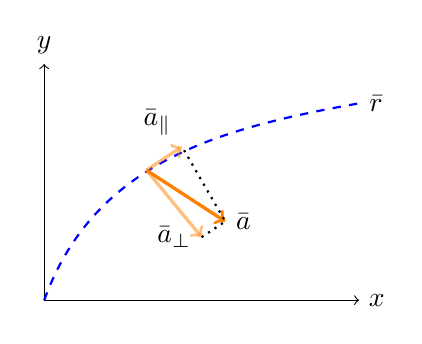
\begin{tikzpicture}
        \draw [<->] (0,3) node [above] {$y$} --(0,0) -- (4,0) node [right] {$x$};
        \draw [thick, dashed, blue] (0,0) to [out=70, in=190] (4,2.5) node [right, black] {$\bar{r}$};
        %\draw [very thick, green, ->] (1.3,1.65) -- (3,2.75) node [above left, black] {$\bar{v}$};
        \draw [very thick, orange, ->] (1.3,1.65) -- (2.3,1) node [right, black] {$\bar{a}$};
        \draw [very thick, orange, opacity=0.5, ->] (1.3,1.65) -- (2,0.8) node [black, opacity=1, left] {$\bar{a}_\perp$};
        \draw [very thick, orange, opacity=0.5, ->] (1.3,1.65) -- (1.75,1.95) node [black, opacity=1, above left] {$\bar{a}_\parallel$};
        \draw [thick, dotted] (2,0.8) -- (2.3,1) -- (1.75,1.95);
    \end{tikzpicture}
\end{document}
